%!TEX root = project.tex

\chapter*{About this project}
% assuming past tense as this report is talking about the completed project
\paragraph{Abstract}
%A brief description of what the project is, in about two-hundred and fifty words.
% leave technical jargon out of it
This project sets out to create a food ordering system for a local company. 
The systems primary components are a mobile application that the user interacts with and a web application that the staff interact with.

The need for such a system stems from two problems, firstly the issue of rush hour times during business hours where there is a vast number of customers to service, and secondly to bring more presence and promotion to the business, as they are finding it hard to reach out to their current customer base and would be customers.

% Mobile app
We aim to solve the first problem by having a system in which customers can pre-order sandwiches and other products via a mobile application.
Users will be able to top up their account, order products, pick a collection time, and view their balance, products and past order history.

The second problem will be solved by implementing push notifications into the application so that the company can let customers know about menus, events and various other updates. Another way to increase promotion and presence is by having various information about the company on the application; for instance: opening times, contact details and general information. 

% web app
All of the information on the web application can be updated; this includes the menus, opening times, user and staff details, and much more. 
This information is reflected in the web application.
Interactions from within the mobile application including: topping up, logging in, registration and ordering go through the web application.

% conclusion
We plan to create a cohesive, thoughtfully designed, robust system that solves these two problems.
\pagebreak

\paragraph{Authors}
%Explain here who the authors are.
This project was created by two fourth year software development students: Ronan Connolly \& Vladislav Marisevs, as part of our Bachelors of Science honours degree in Software Development. 
\linebreak

Ronan was in charge of creating all aspects of the user facing mobile app. 
Vladislav was in charge of creating all aspects of the staff facing web app.

We spent most of our shared time coming up with the overall architecture we would implement, and an interface to be used between mobile and web app for transfer of data.


\pagebreak
\paragraph{Acknowledgements}
We would like to acknowledge and thank our supervisor Dr John Healy for all the time and effort he has put into helping us throughout this project, he gave us a good structure and set milestones for us in order to keep on top of things.
\linebreak

We'd also like to thank the GMIT Catering Company staff for the time spent meeting with us in order to continuously improve and adapt the project.

\chapter{Introduction}	% 3-5 pages
%The introduction should be about three to five pages long.
%Make sure you use references~\cite{einstein}

% should contain a breif intro the the project, how it came about, the reason for it.
% also will break it down into an intro to the latter chapter?

% abstract (change)

%% CONTEXT
% basic idea
We set out to create a food ordering system for the GMIT Catering Company (known henceforth as the company).
The basic structure is a mobile application (henceforth known as mobile app) for the Android and iOS systems that the user interacts with, and a server (henceforth known as web app) that the staff can log into in order to view transactions, user details and to update the mobile app.

% reason #1
The reason such a system is needed is that queues during peak times tend to be enormous and currently it's hard to service all the customers.

% reason #2
Another reason is to encourage customers to get into a habit of repeat ordering, if it is an easy process then it should increase purchases.

% reason #3
Lastly, the company wants to increase presence and promotion in the college, in order to achieve this end we have implemented push notifications where staff can send a notification to all users. On top of this the mobile application itself serves as a promotional device, containing details of various aspects of the company.
\linebreak

%% OBJECTIVES
% mobile app features
The components contained within the mobile app include pages for login, registration, about the company and user details There is also a way to top up and order sandwiches.
A huge emphasis is put on design for this project, using the companies colour theme and creating a nice icon.
% tech
This mobile app was created using the Ionic Framework which is programmed primarily using the AngularJS framework.

% web app features
The components contained within the web app include many pages such as the login system, orders, stock, user details, vouchers(for adding credit to your account), settings(collection and opening times) and accounts(staff) pages.
%tech
This web app was created in PHP using Zend Framework 2.
% reflection in app
Most of the information on the web app is reflected on the mobile app.

% connect the apps
The two applications talk to each other via JSON over HTTP Get and Post requests. 

% conclusion
We set out to create a well thought out, carefully designed, robust food ordering system using modern technologies.
This project could be extended in the future to be used 
\linebreak

% authors (change)
% mention how to laid it out between us
% We thought out, designed and carefully laid out this project into many smaller components.
%Ronan was in charge of creating all aspects of the user facing mobile app. 
%Vladislav was in charge of creating all aspects of the staff facing web app.


% mention agile
We used an agile structure where we had certain components we needed complete by specific dates.
% mention meetings
We had various meetings each month with our supervisor and several members of the company.

%% CHAPTER SUMMARIES


%% GITHUB URLS
%% Web App

%% Mobile App

% main link

% test server link

% push link

\chapter{Context}	% 3-5 pages
\begin{itemize}
\item Provide a context for your project.
\item Set out the objectives of the project
\item Briefly list each chapter / section and provide a 1-2 line description of what each section contains.
\item List the resource URL (GitHub address) for the project and provide a brief list of the main elements at the URL.
\end{itemize}

\section{Filler}
Lorem ipsum dolor sit amet, consectetur adipiscing elit. Etiam mi enim, interdum ut elit lobortis, bibendum tempus diam. Etiam turpis ex, viverra tristique finibus nec, feugiat at metus. Curabitur tempus gravida interdum. Donec ac felis a lorem scelerisque elementum. Vestibulum sit amet gravida tortor, a iaculis orci. Nam a molestie augue. Curabitur malesuada odio at mattis molestie. In hac habitasse platea dictumst. Donec eu lectus eget risus hendrerit euismod nec at orci. Praesent porttitor aliquam diam, eu vestibulum nisl sollicitudin vel. Nullam sed egestas mi.

Quisque vel erat a justo volutpat auctor a nec odio. Sed rhoncus augue sit amet nisl tincidunt, vitae cursus tellus efficitur. Class aptent taciti sociosqu ad litora torquent per conubia nostra, per inceptos himenaeos. Pellentesque et auctor dui. Fusce ornare odio ipsum, et laoreet mi molestie sed. Cras at massa sit amet ipsum gravida aliquam. Nulla suscipit porta imperdiet. Fusce eros neque, bibendum sit amet consequat non, pulvinar quis ipsum.

\subsection{More filler}
Donec fermentum sapien ac rhoncus egestas. Nullam condimentum condimentum eros sit amet semper. Nam maximus condimentum ligula. Praesent faucibus in nisi vitae tempus. Sed pellentesque eleifend ante, ac malesuada nibh dapibus nec. Phasellus nisi erat, pulvinar vel sagittis sed, auctor et magna. Quisque finibus augue elit, consequat dignissim purus mollis nec. Duis ultricies euismod tortor, nec sodales libero pellentesque et. Interdum et malesuada fames ac ante ipsum primis in faucibus.

Donec id interdum felis, in semper lacus. Mauris volutpat justo at ex dignissim, sit amet viverra massa pellentesque. Suspendisse potenti. Praesent sit amet ipsum non nibh eleifend pretium. In pretium sapien quam, nec pretium leo consequat nec. Pellentesque non dui lacus. Aenean sed massa lacinia, vehicula ante et, sagittis leo. Sed nec nisl ac tellus scelerisque consequat. Ut arcu metus, eleifend rhoncus sapien sed, consequat tincidunt erat. Cras ut vulputate ipsum.

Curabitur et efficitur augue. Proin condimentum ultrices facilisis. Mauris nisi ante, ultrices sed libero eget, ultrices malesuada augue. Morbi libero magna, faucibus in nunc vitae, ultricies efficitur nisl. Donec eleifend elementum massa, sed eleifend velit aliquet gravida. In ac mattis est, quis sodales neque. Etiam finibus quis tortor eu consequat. Nullam condimentum est eget pulvinar ultricies. Suspendisse ut maximus quam, sed rhoncus urna.

\section{Filler}
Phasellus eu tellus tristique nulla porttitor convallis. Vestibulum ac est eget diam mollis consectetur. Donec egestas facilisis consectetur. Donec magna orci, dignissim vel sem quis, efficitur condimentum felis. Donec mollis leo a nulla imperdiet, in bibendum augue varius. Quisque molestie massa enim, vitae ornare lacus imperdiet non. Donec et ipsum id ante imperdiet mollis. Nullam est est, euismod sit amet cursus a, feugiat a lectus. Integer sed mauris dolor.

Mauris blandit neque tortor, consequat aliquam nisi aliquam vitae. Integer urna dolor, fermentum ut iaculis ut, semper eu lacus. Curabitur mollis at lectus at venenatis. Donec fringilla diam ac risus imperdiet suscipit. Aliquam convallis quam vitae turpis interdum, quis pharetra lacus tincidunt. Nam dictum maximus lectus, vitae faucibus ante. Morbi accumsan velit nec massa tincidunt porttitor. Nullam gravida at justo id viverra. Mauris ante nulla, eleifend vitae sem vitae, porttitor lobortis eros.

Cras tincidunt elit id nisi aliquam, id convallis ex bibendum. Sed vel odio fringilla, congue leo quis, aliquam metus. Nunc tempor vehicula lorem eu ultrices. Curabitur at libero luctus, gravida lectus sed, viverra mi. Cras ultrices aliquet elementum. Pellentesque habitant morbi tristique senectus et netus et malesuada fames ac turpis egestas. Sed metus ante, suscipit sit amet finibus ut, gravida et orci. Nunc est odio, luctus quis diam in, porta molestie magna. Interdum et malesuada fames ac ante ipsum primis in faucibus. Mauris pulvinar lacus odio, luctus tincidunt magna auctor ut. Ut fermentum nisl rhoncus, tempus nulla eget, faucibus tortor. Suspendisse eu ex nec nunc mollis pulvinar. Nunc luctus tempus tellus eleifend porta. Nulla scelerisque porttitor turpis porttitor mollis.

Duis elementum efficitur auctor. Nam nisi nulla, fermentum sed arcu vel, posuere semper dui. Fusce ac imperdiet felis. Aenean quis vestibulum nisl. Integer sit amet tristique neque, at suscipit tortor. Morbi et placerat ante, vel molestie dui. Vivamus in nibh eget massa facilisis accumsan. Nunc et purus ac urna fermentum ultrices eget sit amet justo. Class aptent taciti sociosqu ad litora torquent per conubia nostra, per inceptos himenaeos. Cras elementum dui nunc, ac tempor odio semper et. Ut est ipsum, sollicitudin eleifend nisl eu, scelerisque cursus nunc. Nam at lectus vulputate, volutpat tellus vel, pharetra mauris. Integer at aliquam massa, at iaculis sem. Morbi nec imperdiet odio. In hac habitasse platea dictumst.

Mauris a neque lobortis, venenatis erat ut, eleifend quam. Nullam tincidunt tellus quis ligula bibendum, a malesuada erat gravida. Phasellus eget tellus non risus tincidunt sagittis condimentum quis enim. Donec feugiat sapien sit amet tincidunt fringilla. Vivamus in urna accumsan, vehicula sem in, sodales mauris. Aenean odio eros, tristique non varius id, tincidunt et neque. Maecenas tempor, ipsum et sollicitudin rhoncus, nibh eros tempus dolor, vitae dictum justo massa in eros. Proin nec lorem urna. In ullamcorper vitae felis sit amet tincidunt. Maecenas consectetur iaculis est, eu finibus mi scelerisque et. Nulla id ex varius, ultrices eros nec, luctus est. Aenean ac ex eget dui pretium mattis. Ut vitae nunc lectus. Proin suscipit risus eget ligula sollicitudin vulputate et id lectus.

\chapter{Methodology}	% 1-2 pages
About one to two Pages

Describe the way you went about your project:
\begin{itemize}
\item Agile / incremental and iterative approach to development. Planning, meetings.
\item What about validation and testing? Junit or some other framework.
\item If team based, did you use GitHub during the development process.
\item Selection criteria for algorithms, languages, platforms and technolo-gies.
\end{itemize}
Check out the nice graphs in Figure \ref{tikz:graphs}, and the nice diagram in Figure \ref{tikz:mydiagram}.

\begin{figure}
	\centering
	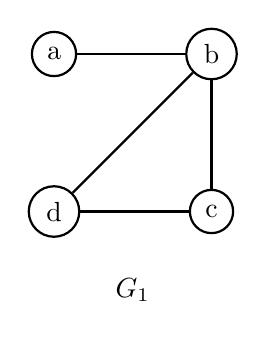
\begin{tikzpicture}
	\begin{scope}[every node/.style={circle,thick,draw}]
	\node (a) at (0,2) {a};
	\node (b) at (2,2) {b};
	\node (c) at (2,0) {c};
	\node (d) at (0,0) {d};
	\end{scope}
	\begin{scope}[every edge/.style={draw=black,thick}]
	\path (a) edge (b);
	\path (b) edge (c);
	\path (b) edge (d);
	\path (c) edge (d);
	\end{scope}
	\node () at (1,-1) {$G_1$};
	\end{tikzpicture}
	\hspace{1.5cm}
	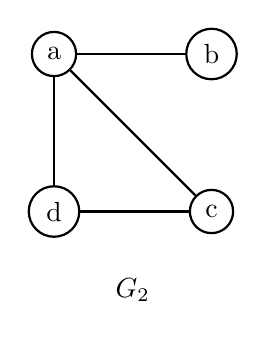
\begin{tikzpicture}
	\begin{scope}[every node/.style={circle,thick,draw}]
	\node (1) at (0,2) {a};
	\node (2) at (2,2) {b};
	\node (3) at (2,0) {c};
	\node (4) at (0,0) {d};
	\end{scope}
	\begin{scope}[every edge/.style={draw=black,thick}]
	\path (1) edge (2);
	\path (1) edge (3);
	\path (1) edge (4);
	\path (3) edge (4);
	\end{scope}
	\node () at (1,-1) {$G_2$};
	\end{tikzpicture}
	\caption{Nice pictures}
	\label{tikz:graphs}
\end{figure}

\begin{figure}
	\centering
	\begin{tikzpicture}[node distance=6cm]
%	\node (a) [rect] {A Big Blue Block};
%	\node[rect](name)
	\node (a) at (4,2) [draw,thick,minimum width=2cm,minimum height=2cm, blue] {A Big Blue Block};
	\node (b) [oval, right of=a] {And His Oval Friend};
	\draw [line] (a) -- (b);
	\end{tikzpicture}
	\caption{Nice pictures}
	\label{tikz:graphs}
\end{figure}


\chapter{Technology Review}	% 7-10 pages
About seven to ten pages.
\begin{itemize}
\item Describe each of the technologies you used at a conceptual level. Standards, Database Model (e.g. MongoDB, CouchDB), XMl, WSDL, JSON, JAXP.
\item Use references (IEEE format, e.g. [1]), Books, Papers, URLs (timestamp) – sources should be authoritative. 
\end{itemize}

\section{Web App}	% 4 pages
I decided to use PHP since I was already proficient at it and it works really well as a web app because....

\subsection{PHP}

\subsection{Zend Framework}

\pagebreak

\section{Mobile App} % 4 pages
\subsection{Ionic Framework}
% talk about JS, AngularJS, CSS, HTML and Ionic.
\subsubsection{HTML/CSS}

\subsubsection{JavaScript}

\subsubsection{AngularJS}
Here's some nicely formatted XML:
\begin{minted}{xml}
	<this>
	<looks lookswhat="good">
	Good
	</looks>
	</this>
\end{minted}

\subsection{Alternatives}
% alternatives? JQueryPhone, PhoneGap, Cordova, Xamarin
\subsubsection{Cordova}

\subsubsection{PhoneGap}

\subsubsection{JQueryMobile}

\subsubsection{Xamarin}

\section{REST Architecture}	% 1/2 pages
\subsection{HTTP Requests}
% talk about the HTTP get/post requests used via the interface from the phone and server
\subsection{Custom API}
% The web server has a custom API that the mobile app uses

\section{JSON}	% 1 pages

\chapter{System Design}	% n-m pages
As many pages as needed.
\begin{itemize}
\item Architecture, UML etc. An overview of the different components of the system. Diagrams etc… Screen shots etc.
\end{itemize}

\begin{table}[h]
  \centering
  \begin{tabular}{x{2cm}p{3cm}}
    \toprule \\
    Column 1 & Column 2 \\
    \midrule \\
    Rows 2.1 & Row 2.2 \\
    \bottomrule
  \end{tabular}
  \caption{A table.}
  \label{table:mytable}
\end{table}

\chapter{System Evaluation}	% n-m pages
As many pages as needed.
\begin{itemize}
\item Prove that your software is robust. How? Testing etc. 
\item Use performance benchmarks (space and time) if algorithmic.
\item Measure the outcomes / outputs of your system / software against the objectives from the Introduction.
\item Highlight any limitations or opportuni-ties in your approach or technologies used.
\end{itemize}

\chapter{Conclusion}	% 1-3 pages
About three pages.

\begin{itemize}
\item Briefly summarise your context and ob-jectives (a few lines).
\item Highlight your findings from the evalua-tion section / chapter and any opportuni-ties identified.
\end{itemize}

